\subsection{Aufbau der Datenpakete}
\subsubsection{Überblick}
Es handelt sich bei dem zu entwickelnden Protokoll um ein Nachrichtenprotokoll. Daher wird der aus anderen Protokollen bekannte Begriff Datenpaket hier als eine Nachricht (Message) definiert. Diese Nachricht wird in zwei Hauptteile gegliedert. Den ersten Teil bildet der Nachrichtenheader, während der zweite Teil durch eine Instanz der Klasse \textit{Knowledge} gebildet wird.
\begin{figure}[H]
	\centering
	\hspace*{1cm}
	\makebox[\linewidth][c]{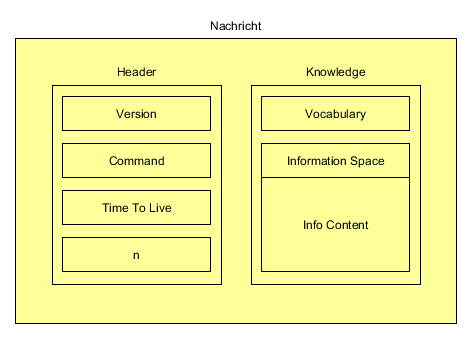
\includegraphics[width=1.0\linewidth]{entwurf/images/NachrichtAufbau1.png}}%
	\caption{Die zwei Hauptbestandteile einer Nachricht}
	\label{fig:message1}
\end{figure}
\subsubsection{Header}
Der Nachrichtenheader wird im Gegensatz zu anderen klassischen Routingprotokollen nicht zum Routing eingesetzt, dies ist allein von den semantischen Annotationen innerhalb des \textit{Knowledge} abhängig. Der Header ist dennoch unabdingbar, da er eine Nachricht als SharkNet Broadcast-Nachricht kennzeichnet und die Verarbeitungsart der Nachricht kennzeichnet. Der Header enthält folgende Bestandteile:
\begin{table}[H]
	\begin{center}
		\caption{Bestandteile des Headers}
		\label{tab:messageHeader}
		\begin{tabular}{l|l} 			
			Bestandteil & Erläuterung \\
			\hline
			Version & aktuelle Version des Protokolls\\
			Format & Format der Nachricht, standardmäßig JSON\\
			TTL & Time To Live Wert der Nachricht\\
			Command & Verarbeitungsart der Nachricht, Insert oder Expose\\
			Physical Sender & Absender der Nachricht\\
			Receiver Peer & Zielgerät der Nachricht\\
			Receiver Location & Ort des Absenders beim Versenden der Nachricht\\
			Receiver Time & Zeitpunkt des Absendens der Nachricht\\
			Topic & Sequenznummer, wird nicht vom semantischen Filter ausgewertet\\
			Type & Kennzeichnung der Nachrichtenart\\							
		\end{tabular}
	\end{center}
\end{table}
Die obligatorischen Headerbestandteile sind: Version, Format, Command, Receiver Peer und Type. Der Command ist für das Versenden der Nachrichten auf \textit{Insert} gestellt, damit die Empfangsgeräte die neue Nachricht nach erfolgreicher Filterung in ihre Wissensbasis einfügen. Der zweite Command \textit{Expose} wird fast ausschließlich von der WiFi-Komponente zum Austausch von Kontaktinformationen benutzt. Auch wenn es sich um einen Broadcast handelt, muss das Zielgerät stets im Header eingetragen sein, die Nachricht kann sonst nicht zugestellt werden. Wenn sich also beispielsweise fünf Geräte in der Nähe befinden, werden fünf Nachrichten mit angepasstem Header verschickt. Der Type markiert die Nachricht als eine Broadcast-Nachricht, damit diese nicht fälschlicherweise als Chat-Nachricht verarbeitet wird.
\subsubsection{Knowledge}
Der Hauptteil der Nachricht spaltet sich in drei Bereiche auf.
\begin{itemize}
	\item Das Vocabulary, welches alle Semantic Tags beinhaltet, die die Nachricht beschreiben
	\item Einen Informationsraum (InformationSpace), der die semantische Beschreibung des Nachrichteninhalts ist. Er besteht aus den in Kapitel zwei beschriebenen sieben Dimensionen mit den dazugehörigen Semantischen Netzen.
	\item Der eigentliche Nachrichteninhalt (Info Content)	
\end{itemize}
Der in Abbildung 3.1 dargestellte Bereich \textit{Info Meta Data} befindet daher sich wie oben beschrieben im Header und nicht im Knowledge.
\subsection{Nachrichtenaustausch}
\subsubsection{Ohne semantische Filterung}
Der Austausch von Nachrichten mittels des Protokolls erfolgt zunächst ungerichtet an alle Kommunikationsteilnehmer, die sich in Reichweite befinden. Jeder Teilnehmer entscheidet selbst, ob er eine Nachricht seiner Wissensbasis hinzufügt und sie ebenfalls an alle in der Nähe befindlichen Geräte sendet. Wie im Kapitel Grundlagen beschrieben, müssen dabei Loops unterbunden werden, da die Kommunikation sonst durch eine Endlosschleife fehschlagen würde. Das folgende Szenario stellt beispielhaft diese Situation ohne Beachtung einer semantischen  Filterung dar.
\begin{figure}[H]
	\centering
	\hspace*{1cm}
	\makebox[\linewidth][c]{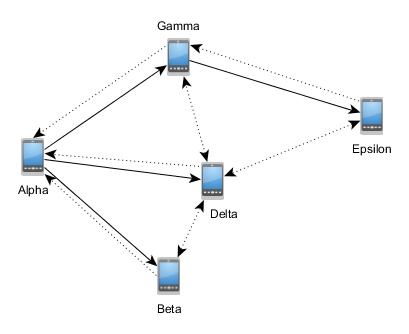
\includegraphics[width=0.6\linewidth]{entwurf/images/beispielszenario.png}}%
	\caption{Kommunikation ohne semantische Filterung}
	\label{fig:beispielszenario}
\end{figure}
Das Szenario von Abbildung 4.2 beinhaltet die fünf Smartphones Alpha, Beta, Gamma, Delta und Epsilon, welche zusammen ein kabelungebundenes Ad-hoc-Netz bilden. Der Urpsrung der Nachricht ist Alpha, welches eine Nachricht per Broadcast an alle Geräte schickt. Es befinden sich jedoch nur die Geräte Gamma, Delta und Beta in der direkten Reichweite von Alpha. Alpha sendet zunächst an alle Geräte in Reichweite die Nachricht, was jeweils durch die durchgezogene Kante symbolisiert wird. Die Geräte Gamma, Delta und Beta senden nun ihrerseits die empfangene Nachricht an alle Geräte in Reichweite. Dies würde jedoch zu Schleifen innerhalb der Kommunikation führen, falls bereits empfangene oder abgeschickte Nachrichten nicht abgelehnt werden sollten. Dies wird mit gepunkteten Kanten symbolisiert. Eine Ausnahme ist die Nachricht, die von Gamma an Epsilon geschickt wird. Da Epsilon keine Nachricht von Alpha empfangen konnte, wird die Nachricht von Gamma akzeptiert. 
\subsubsection{Mit semantischer Filterung}
Der Standardfall für die zu entwickelnde Anwendung wird der wiederholte Broadcast mit vorhergehender und nachfolgender semantischer Filterung sein. Jedes Gerät kann durch einen Eingangsfilter und einen Ausgangsfilter festlegen, welche Nachrichten akzeptiert und eventuell zusätzlich an andere Geräte in der Nähe weitergeleitet werden. 
\\Sollte beispielsweise Alpha eine Nachricht versenden, die nicht den Eingangsfilter von Gamma passieren kann, würde sich der eben vorgestellte Kommunikationsablauf nun wie folgt darstellen.
\begin{figure}[H]
	\centering
	\hspace*{1cm}
	\makebox[\linewidth][c]{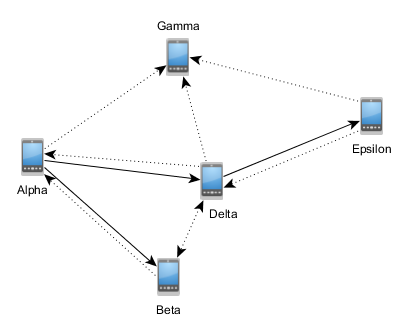
\includegraphics[width=0.6\linewidth]{entwurf/images/beispielszenario2.png}}%
	\caption{Kommunikation mit semantischer Filterung I}
	\label{fig:beispielszenario2}
\end{figure}
Gamma lehnt die Nachricht aufgrund seines Filters ab, dabei ist es unerheblich von welchem Gerät die Nachricht kommt. Folglich kann Epsilon die Nachricht nicht mehr von Gamma erhalten, stattdessen wird diese nun von Delta empfangen. 
\\Falls mehrere Geräte einen restriktiven Eingangsfilter konfiguriert haben, können Nachrichten teilweise nicht an alle Geräte zugestellt werden, wie das folgende Szenario zeigt.
\begin{figure}[H]
	\centering
	\hspace*{1cm}
	\makebox[\linewidth][c]{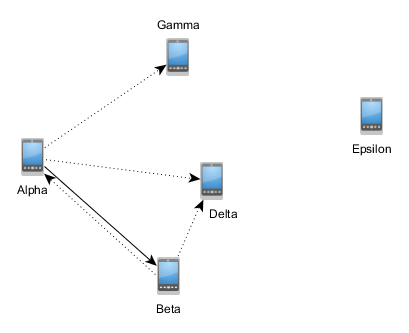
\includegraphics[width=0.6\linewidth]{entwurf/images/beispielszenario3.png}}%
	\caption{Kommunikation mit semantischer Filterung II}
	\label{fig:beispielszenario3}
\end{figure}
In diesem Szenario lehnen sowohl Gamma als auch Delta die Nachricht ab, nur Beta akzeptiert die Nachricht und versucht diese weiterzuleiten. Da Epsilon sich nicht innerhalb der Sendereichweite von Alpha oder Beta befindet, kann die Nachricht das Gerät nicht erreichen. Die Anzahl der Routen wurde durch die Filterung also deutlich verringert. 
\\Dies mag zunächst problematisch erscheinen, ist aber die Intention des Protokolls. Das hier vorgeschlagene inhaltsbasierte Routing hat nicht das vorrangige Ziel, effiziente Routen zu allen Geräten zu finden, sondern soll allein von den Interessen der Geräte abhängig sein. 

\subsection{Ablauf der Filterung}
Um einen adäquaten Aufbau und Ablauf der Filterung bestimmten zu können, müssen zunächst die Anforderungen an den Filter formuliert werden.
\begin{itemize}
	\item Es müssen alle Dimensionen (siehe Abbildung 3.1) ausgewertet werden können, die im Shark-Framework/ASIP definiert sind.
	\item Weiterhin muss dynamisch einstellbar sein, wann welche Dimension durch den Filter ausgewertet wird. Es muss auch nicht zwingend jede Dimension ausgewertet werden, dies ist ebenfalls abhängig vom Benutzer.
	\item Die Auswertung sollte nur mit Datenstrukturen ausgeführt werden, die aus dem Shark-Framework/ASIP bekannt sind.
	\item Die Filterung findet nach dem Erhalt der Nachricht und vor der Anzeige auf dem Gerät statt. Der Prozess der Filterung ist daher sehr zeitkritisch und muss möglichst schnell durchgeführt werden können. Sollte ein vom Eingangsfilter abweichender Ausgangsfilter gesetzt sein, muss die Nachricht sogar zweimal gefiltert werden.
	\item Es muss unbedingt mit Interfaces gearbeitet werden, um die Erweiterbarkeit und Austauschbarkeit des Filterprozesses zu gewährleisten.
\end{itemize}
Eine Implementierung des Filters muss diese Punkte beachten, in der Komponentenbeschreibung des semantischen Filters finden sich Details zu der im Rahmen dieser Arbeit erstellten Implementierung. [...]
\\Das folgende Aktivitätsdiagramm skizziert den Ablauf des Nachrichtenempfangs.
\begin{figure}[H]
	\centering
	\hspace*{1cm}
	\makebox[\linewidth][c]{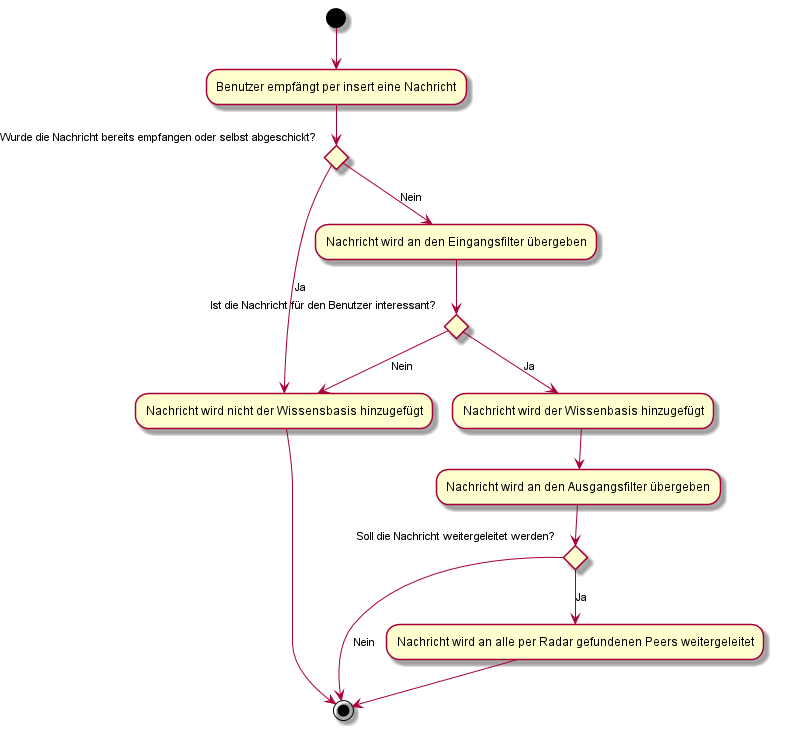
\includegraphics[width=1.0\linewidth]{entwurf/images/empfangNachricht.png}}%
	\caption{Filterung nach dem Empfang einer Nachricht}
	\label{fig:empfangNachricht}
\end{figure}
Hierbei wird auch ersichtlich, dass vor der eigentlichen Filterung bereits empfangene oder versandte Nachrichten nicht verwertet werden dürfen, um die Bildung von Schleifen zu vermeiden. Die verschiedenen technischen Umsetzungen zur Schleifenvermeidung wurden im Unterkapitel Broadcast-Routing erläutert. 
\\Für die Implementierung wurde zur Schleifenvermeidung eine Abwandlung des sequenznummerkontrollierten Floodings (SNKF) gewählt (siehe dazu auch die Komponentenbeschreibung des Broadcasts). Es hat den Vorzug vor dem \textit{Reverse Path Forwarding} (RPF) und dem \textit{Spanning Tree} aus den folgenden Gründen erhalten:
\begin{itemize}
	\item Der Spanning Tree muss nach jeder topologischen Änderung neu aufgebaut werden. Dies ist bei aus Smartphones bestehenden Ad-Hoc-Netzwerken häufig der Fall, da davon auszugehen ist, dass sie von sich stetig bewegenden Menschen getragen werden. Der Aufwand für den wiederholten Aufbau des Spanning Trees ist dementsprechend hoch.
	\item Vor dem gleichen Problem steht das RPF. Die Bestimmung des kürzesten Pfades gestaltet sich schwierig, wenn die beteiligten Geräte nicht stationär sind. Bei Geräten in Bewegung besteht die Gefahr, dass Nachrichten ungewollt abgelehnt werden.
	\item Im Gegensatz dazu muss beim SNKF nur eine Tabelle pro Gerät gepflegt werden, in der die Sequenznummern der Nachrichten gespeichert werden und diese unabhängig von der Topologie ist. Bereits empfangene oder versandte Nachrichten können durch die Sequenznummer erkannt und die Bearbeitung folglich abgelehnt werden.
\end{itemize}
Die Sequenznummer ist für das Protokoll eindeutig in Form einer Zeichenkette definiert. Diese Zeichenkette enthält zum einen den \textit{Subject Identifier} des Urhebers der Nachricht und zum anderen den genauen Zeitpunkt der Erzeugung der Nachricht. Diese generierte Sequenznummer ist, wie in Tabelle 4.1 dargestellt, Teil des Headers der Nachricht und wird nach Erhalt der Nachricht mit der Tabelle abgeglichen. 
\subsection{Architektur}
Die Android-Anwendung SharkNet bindet das SharkFramework als .jar Datei ein. In beiden Teilbereichen wurden für die praktische Umsetzung des semantischen Broadcasts Klassen hinzugefügt. Der Aufbau der Anwendung folgt dabei dem Model-View-Control Entwicklungsmuster, was mit Hilfe von einander getrennten Activitites, Services, Datenzugriffsobjekten (DAO) und Entitäten umgesetzt worden ist. Das grundlegende Zusammenwirken der zu entwickelnden Klassen zwischen Anwendung und Framework lässt sich beispielhaft an zwei einfachen Szenarios erklären. Beim ersten Beispiel schreibt der Benutzer eine Broadcast-Nachricht.
\begin{figure}[H]
	\centering
	\hspace*{1cm}
	\makebox[\linewidth][c]{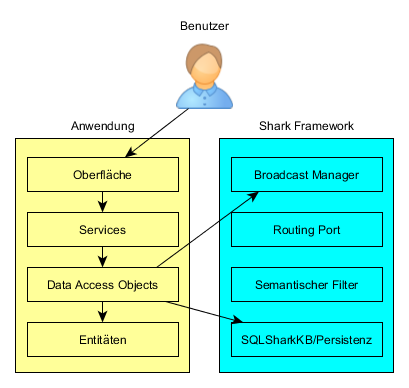
\includegraphics[width=0.7\linewidth]{entwurf/images/strukturNachrichtSenden.png}}%
	\caption{Anwendung und Framework beim Absenden einer Nachricht}
	\label{fig:sendenNachrichtStruktur}
\end{figure}
\begin{enumerate}
	\item Der Benutzer gibt über die Benutzeroberfläche eine Broadcast-Nachricht ein und sendet diese ab. 
	\item Der zuständige Service nimmmt die Zeichenkette entgegen, führt eine \textit{sanitization} durch und reicht diese an ein DAO weiter
	\item Das DAO erhält vom Service eine Message-Entität. Es ist zuständig für das Speichern, Löschen und Editieren von Entitäten. Das DAO nutzt nun die \textit{SQLSharkKB}, um das Objekt der Wissensbasis des Benutzers hinzuzufügen. 
	\item Die SQLSharkKB speichert nun die Entität innerhalb einer SQLite-Datenbank. Sie wird im Unterkapitel Persistenz näher erläutert.
	\item Nachdem die Nachricht gespeichert worden ist, soll sie an alle Geräte in der Umgebung versandt werden. Dies geschieht durch den \textit{Broadcast Manager}, welcher die Nachricht vom DAO entgegen nimmt und sie per WiFi-Direct und Bluetooth versendet.
\end{enumerate}
Der Routing Port und der Semantische Filter sind nur beim Empfangen von Nachrichten relevant. Beim Empfang kehrt sich der Ablauf gewissermaßen um, die Nachricht wandert vom Framework zur Anwendung. 
\begin{figure}[H]
	\centering
	\hspace*{1cm}
	\makebox[\linewidth][c]{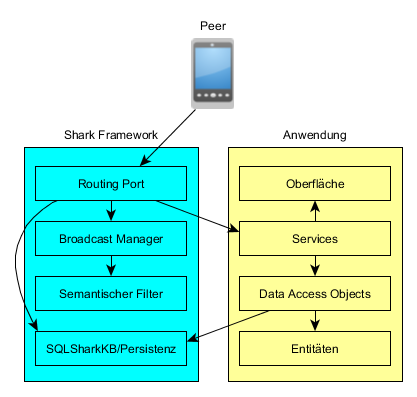
\includegraphics[width=0.7\linewidth]{entwurf/images/strukturNachrichtEmpfangen.png}}%
	\caption{Anwendung und Framework beim Absenden einer Nachricht}
	\label{fig:empfangenNachrichtStruktur}
\end{figure}
\begin{enumerate}
	\item Das Gerät empfängt vom Smartphone Beta eine Broadcast-Nachricht. Dies wird zunächst vom \textit{Routing Port} verwertet, welcher die beiden aus dem Kapitel Grundlagen bekannten Methoden \textit{insert()} und \textit{expose()} implementiert. Beim Nachrichteneingang wird nun die Methode \textit{insert()} ausgeführt.
	\item Der \textit{Routing Port} lässt vom \textit{Broadcast Manager} prüfen, ob die Nachricht bereits empfangen oder abgeschickt worden ist per Sequenznummernvergleich.
	\item Sollte die nachricht noch nicht empfangen worden sein, überprüft nun der Semantische Filter, ob die Nachricht für den Empfänger interessant ist. Die Komponentenbeschreibung Semantischer Filter beschreibt die Umsetzung des Filters innerhalb der Anwendung. 
	\item Der \textit{Routing Port} fügt nun die Nachricht der Wissensbasis hinzu und lässt dies von der \textit{SQlSharkKB} persistieren, falls die Nachricht für den Benutzer interessant sein sollte.
	\item Per Listener wird die Nachricht anschließend von der Framework-Ebene auf die Anwendungsebene übermittelt, indem der Service eine Benachrichtigung über neue Nachrichten innerhalb der Wissensbasis erhält. 
	\item Der Service lässt vom DAO aus der Wissensbasis die Broadcast-Nachrichten lesen, diese Liste enthält die alten sowie die neuen Nachrichten.
	\item Die Broadcast-Nachrichten werden auf der Oberfläche angezeigt.
\end{enumerate}

\subsection{Persistenz}
Alle Daten der Anwendung werden innerhalb einer Wissensbasis gespeichert. Das Interface der Wissensbasis ist die \textit{SharkKB}, deren Implementierungen die Daten persistieren. Die offiziell von Android unterstützte Datenbanktechnolgie ist SQLite. Es muss daher eine Implementierung der Shark-Wissensbasis mit SQLite entwickelt werden, um die bereits vorgestellten Strukturen dauerhaft auf Android-Smartphones speichern zu können. 
\\Dafür muss zunächst ein Datenbankschema festgelegt werden. 
\begin{figure}[H]
	\centering
	\hspace*{1cm}
	\makebox[\linewidth][c]{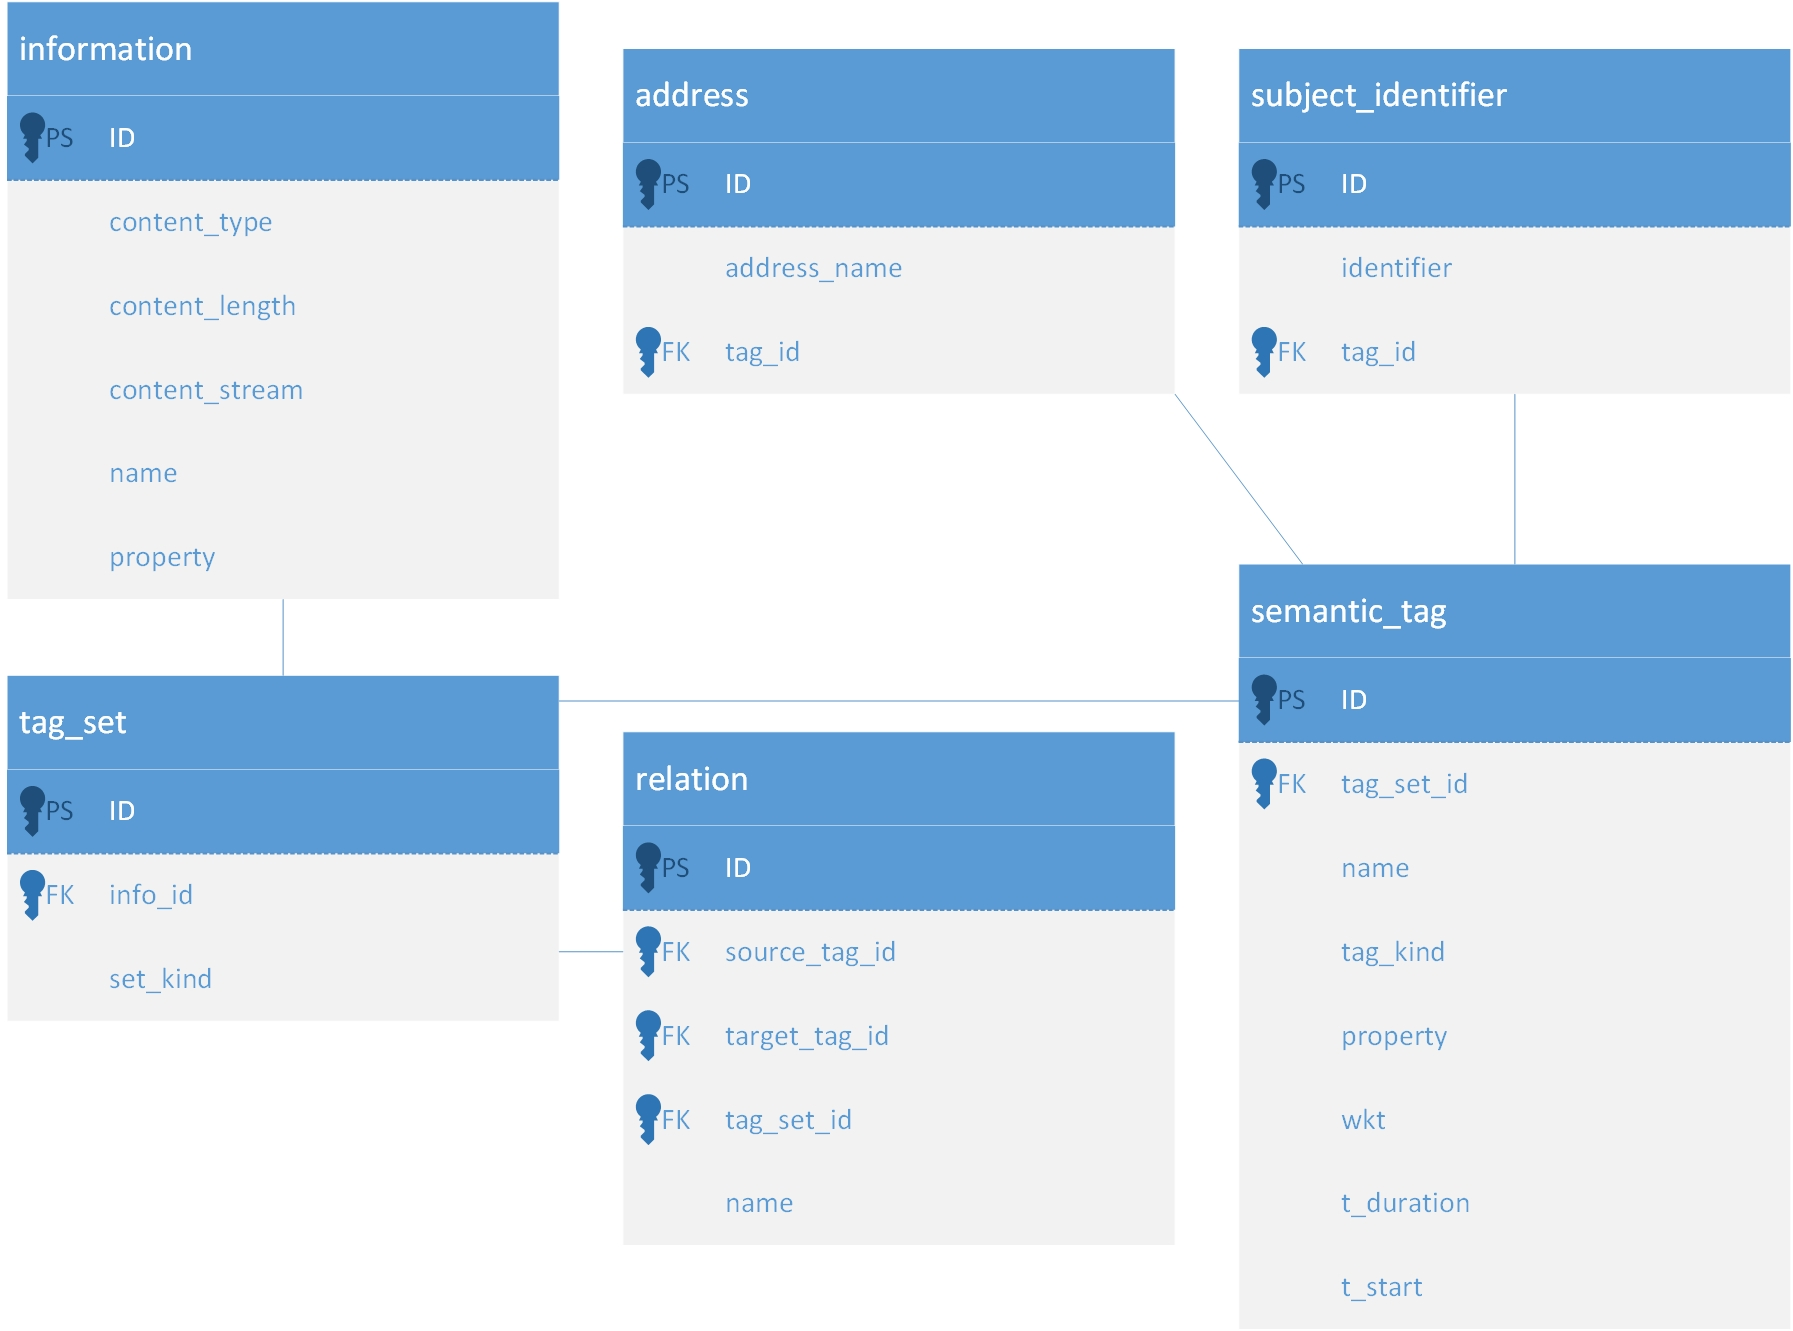
\includegraphics[width=0.8\linewidth]{entwurf/images/sharkSQL.jpg}}%
	\caption{Auszug aus dem Datenbankschema der SQLite Implementierung der SharkKB}
	\label{fig:sharkSQL}
\end{figure}
Alle Tabellen verfügen über eine sich für jeden neuen Eintrag automatisch inkrementierende ID, die als Primärschlüssel dient. \\Die Tabelle \textit{semantic tag} kann jede Art eines \textit{Semantic Tag} darstellen, diese wird durch das Attribut \textit{tag kind} gekennzeichnet (normal, peer, time, spatial). Entsprechend der Art können zusätzliche Attribute gesetzt sein, \textit{wkt} für \textit{Spatial Tags} und duration sowie start für \textit{Time Tags}. Da ein \textit{Semantic Tag} mehrere \textit{Subject Identifier} haben kann, sind diese in einer extra Tabelle ausgelagert. Das gleiche gilt für die Adressen, falls es sich um ein \textit{Peer Semantic Tag} halten sollte. 
\\Die bereits erläuterten Strukturen \textit{Tag Set} und \textit{Semantic Net} werden durch die Tabelle \textit{tag set} repräsentiert. Ähnlich wie beim \textit{Semantic Tag} wird durch das Attribut \textit{set kind} festgelegt, welche der beiden Strukturen ein Eintrag der Tabelle angehört. 
\\Wenn es sich um ein \textit{Semantic Net} handelt, können jeweils zwei Tags durch benannte Beziehungen miteinander verknüpft werden. Diese Beziehung ist über die Fremdschlüssel dann den beiden Tags und dem Semantischen Netz zugeordnet. 
\\Einem \textit{tag set} kann einer Information zugeordnet werden. Die Tabelle \textit{information} enthält unter anderem die Rohdaten der Nachricht (Attribut \textit{conent stream}) und wird durch die zugeordneten \textit{Tag Sets} semantisch eingeordnet. 
\newline [...]

\subsection{Benutzeroberfläche}
Die grafische Benutzeroberfläche muss es dem Benutzer vor allem bei der Eintragung von semantischen Annotationen so simpel wie möglich machen, mit der Anwendung adäquat zu interagieren. Das Design sollte möglichst modern und schlicht sein, wobei es jedoch keinen Schwerpunkt dieser Arbeit darstellen soll. 
\\Die dafür teils von der Chatfunktionalität weitergenutzte und teils neu entwickelte Oberfläche wird nun wieder anhand eines kleinen Beispiels beschrieben. 
\newpage